% Ejemplo de la plantilla de latex para las diapositivas del Máster en IA 

%%%%%%%%%%%%%%%%%%%%%%%%%%%%
%% Valores para el ratio de aspecto: 43, 169 
%\documentclass[10pt, envcountsect, presentation, aspectratio=1610, hyperref={hypertexnames=true}]{beamer}
\documentclass[10pt, envcountsect, handout, aspectratio=1610, hyperref={hypertexnames=true}]{beamer}

%%%%%%%%%%%%%%%%%%%%%%%%%%%%

%%%%%%%%%%%%%%%%%%%%%%%%%%%%
%% Incluir fichero de estilo del máster
\input ../style/plantillaMasterIA.sty
%%%%%%%%%%%%%%%%%%%%%%%%%%%%

\addbibresource{../references.bib}



%\setbeameroption{show only notes} % Only notes
%\setbeameroption{show notes on second screen=right}  % Both
%\setbeamertemplate{note page}[compress]
\setbeameroption{hide notes} % Only slides


\renewcommand*\footnoterule{}
\setbeamerfont{footnote}{size=\tiny}







%\input{embed_video.tex}
%\usepackage{movie15}
\usepackage{multimedia}

%%%%%%%%%%%%%%%%%%%%%%%%%%%%
%% Información que aparecerá en la portada
\title[Aprendizaje por Refuerzo]{Extensiones del Machine Learning}
\subtitle{Introducción al Aprendizaje por Refuerzo} % short title for footer

\author[L. D. Hernández] % Para el pie de página, poner los autores abreviados separados por comas.
{%
	\sc{Luis Daniel Hernández Molinero }\\ % Autor 1
	\textit{Ciencia de la Computación e Inteligencia Artificial}\\  % Area de conocimiento
	\textit{Dept. Ingeniería de la Información y las Comunicaciones}\\  % Departamento
	\\   % No dejes espacio entre esta línea y la llave siguiente 
}

\institute[DIIC]% % Poner las iniciales de los diferentes departamentos de los autores separadas por comas.
{
	\textit{Universidad de Murcia}
}

\date{2024/2025} % Curso académico

\newcounter{yearnext}
\setcounter{yearnext}{\the\year}
\addtocounter{yearnext}{1}

\newcounter{yearprev}
\setcounter{yearprev}{\the\year}
\addtocounter{yearprev}{-1}

\date{\arabic{yearprev} / \the\year\ } % Curso académico

%%%%%%%%%%%%%%%%%%%%%%%%%%%%%%%%%%
%% Contenido de las diapositivas
\setbeamerfont{normal text}{size=\normalsize} % Modifica el tamaño del texto de las diapositivas.
\AtBeginDocument{\usebeamerfont{normal text}}

%%%%%%%%%%%%%%%%%%%%%%%%%%%%%%%%%%

\begin{document}	

%%%%%%%%%%%%%%%%%%%%%%%%%%%%%%%%%%

%%%%%%%%%%%%%%%%%%%%%%%%%%%%%%%%%%

\begin{frame}[plain]
	\titlepage
\end{frame}

%%%%%%%%%%%%%%%%%%%%%%%%%%%%%%%%%%

\begin{frame}{Índice de Contenidos}
	\tableofcontents 
\end{frame}





%%%%%%%%%%%%%%%%%%%%%%%%%%%%%%%%%%
%%%%%%%%%%%%%%%%%%%%%%%%%%%%%%%%%%
\section{Introducción}



%%%%%%%%%%%%%%%%%%%%%%%%%%%%%%%%%%
%%%%%%%%%%%%%%%%%%%%%%%%%%%%%%%%%%
\begin{frame}{Introducción al Aprendizaje por Refuerzo}
\begin{itemize}
	\item \key{Aprender} (RAE) 
	
	\begin{quote}
	Del lat. apprehendĕre. \\
	1. tr. Adquirir el conocimiento de algo por medio del estudio o de la experiencia. \textrm{U. t. c. intr. Hay que aprender de los propios errores.}
	\end{quote}
	
	\begin{itemize}
	\item Nos interesa el conocimiento adquirido desde la experiencia.
	\item Solo se adquiere a través de estímulos (recompensas) de refuerzo.
	\end{itemize}
	
	\item Una definición computacional:
	
	\begin{quote}
	El \key{aprendizaje por refuerzo} consiste en \textbf{aprender} de forma dirigida qué acciones debe escoger un agente software \textbf{interactuando} con el entorno, usando situaciones de aprendizaje idealizadas, \textbf{maximizando} alguna noción de ``recompensa'' o premio acumulado.
	\end{quote}
	
	
\item \textbf{Contexto histórico:}
    \begin{itemize}
        \item Aprendizaje por Ensayo y Error: \textit{Ley de Efecto (Edward Thorndike, 1900)} 
        	\href{https://www.youtube.com/watch?v=fanm--WyQJo}{\large \texttwemoji{film projector}}

        
        	\begin{quote}
			\it Cualquier comportamiento que es seguido por consecuencias agradables es probable que se repita y cualquiera que sea seguido por  consecuencias desagradables es probable que sean evitadas.
			\end{quote}
			
	
        \item Teoría del Control Óptimo: \qquad
        \raisebox{-0.7\height}{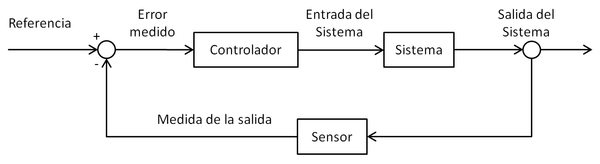
\includegraphics[width=.6\textwidth, height=.2\textheight]{fig/ControlLazo.png}}

    \end{itemize}
\end{itemize}


\end{frame}




%%%%%%%%%%%%%%%%%%%%%%%%%%%%%%%%%%
%%%%%%%%%%%%%%%%%%%%%%%%%%%%%%%%%%


\begin{frame}{¿Quién Estudia el RL?}{\cite{silver2015}}

\begin{center}
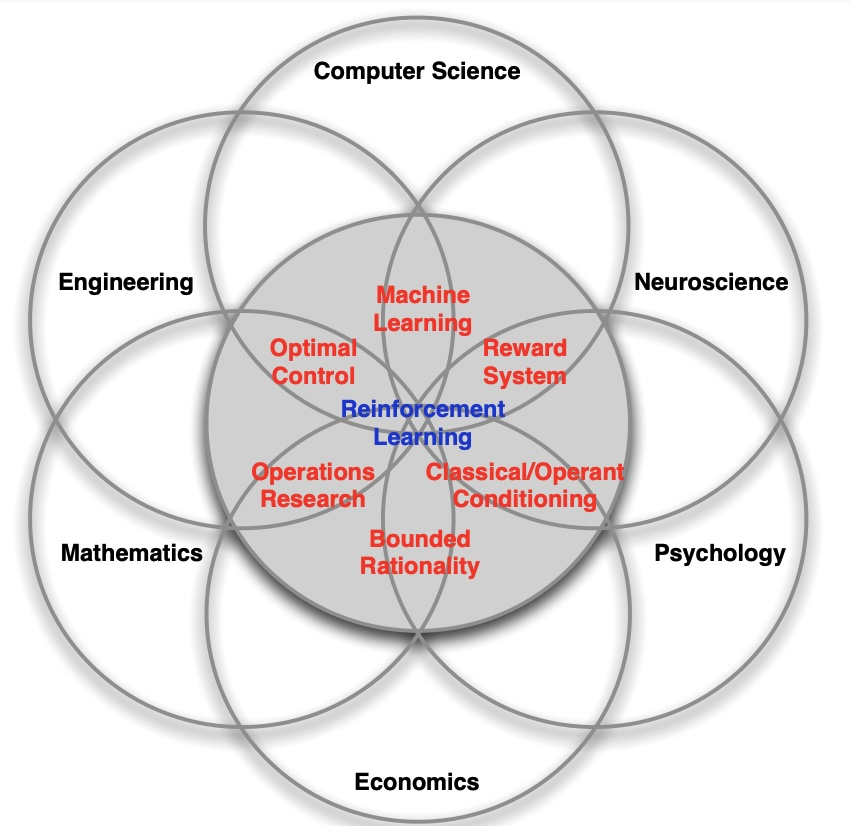
\includegraphics[width=.5\textwidth]{fig/carasRL}
\end{center}

\end{frame}    





%%%%%%%%%%%%%%%%%%%%%%%%%%%%%%%%%%
%%%%%%%%%%%%%%%%%%%%%%%%%%%%%%%%%%
\begin{frame}{Aprendizaje por Refuerzo es otro Tipo de Aprendizaje}{\cite{silver2015}}

\begin{columns}
\begin{column}{.5\textwidth}
\begin{center}
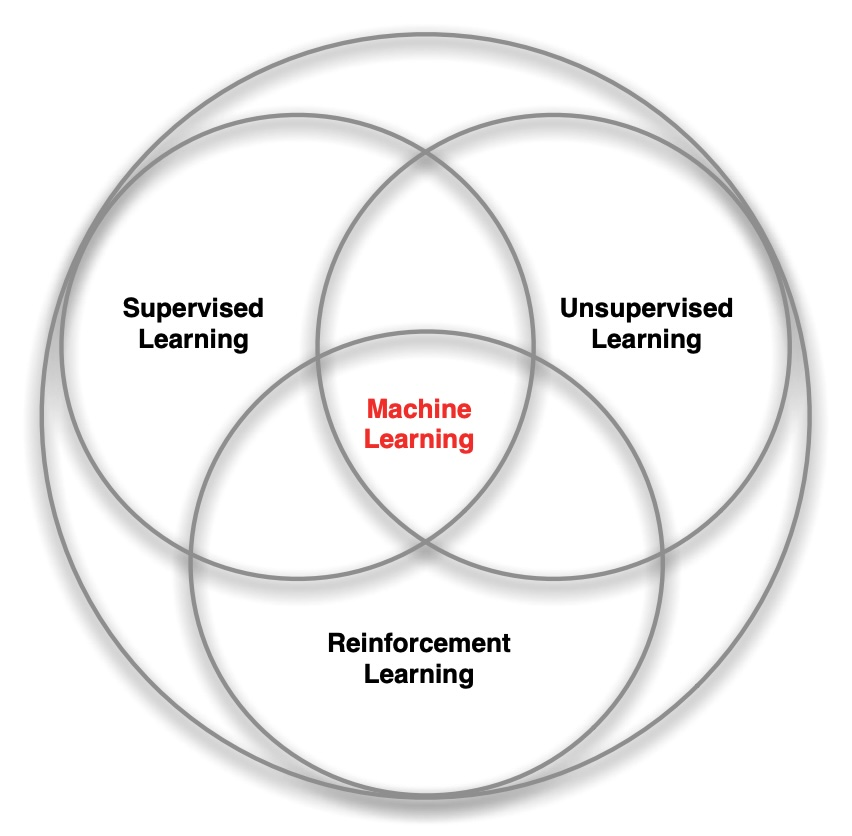
\includegraphics[width=\textwidth]{fig/diagramaML}
\end{center}
\end{column}
\begin{column}{.5\textwidth}
\begin{itemize}
\item \key{Supervisado:} Aprender de un conjunto de datos con sus salida (etiquetas).

\begin{itemize}
\item[P.e.] Clasificar los datos en base a categorías conocidas.
\end{itemize}

\item \key{No supervisado:} Aprender una estructura oculta a partir de datos no etiquetados.

\begin{itemize}
\item[P.e.]  Agrupar datos similares sin que se tenga una categoría predefinida.
\end{itemize}

\item \key{Aprendizaje por refuerzo: }
\begin{itemize}
\item No aprende de datos iid.
\item Aprender de la exploración vs explotación
\item Aprender del entorno (agente interactivo)
\end{itemize}

\end{itemize}
\end{column}
\end{columns}



\end{frame}



%%%%%%%%%%%%%%%%%%%%%%%%%%%%%%%%%%
%%%%%%%%%%%%%%%%%%%%%%%%%%%%%%%%%%
\begin{frame}{Algunos Ejemplo (de Control)}

\begin{itemize}
\item \href{https://youtu.be/e0Lvw6cyug8?si=_L4XlD2mmgby_Vm2&t=145}{Ponerse en pie} una gacela recién nacida.

\begin{itemize}
\item Se pone en pie en menos de 30' y está corriendo en una hora.
\end{itemize}

\item \key{Sistemas de control} (adaptativo) industrial.

\begin{itemize}
\item Controla un sistema en tiempo real sin supervisión humana (p.e. una refinería).
\end{itemize}



\item Gestionar un portafolio de inversiones.

\begin{itemize}
\item Debe decidir sobre cuánto invertir y en qué. P.e.  \citep{Uta2022Portafolio}, 
\end{itemize}



\item \key{Control de aeronaves. }

\begin{itemize}
\item Controlar cada una de las piruetas acrobáticas que pueden hacer un helicóptero \citep{ng2004inverted} \href{https://www.youtube.com/watch?v=Idn10JBsA3Q}{\large \texttwemoji{film projector}}

\item Controlar un planeador usando corrientes calientes de aire \citep{linn2017science}
 \href{https://www.youtube.com/watch?v=daINKmR1M-4}{\large \texttwemoji{film projector}}

\end{itemize}


\item \key{Jugar} al juego de backgammon, go, shogi, ajedrez, .... 

\begin{itemize}
\item \href{https://en.wikipedia.org/wiki/TD-Gammon}{TD-Gammon} de  Gerald Tesauro ganó en 1998 al campeón del mundo.

\item Alpha-Go de \citep{silver2016mastering} 
\href{https://youtube.com/playlist?list=PLqYmG7hTraZBy7J_4ynYPc0Ml1RUGcLmD&si=yry-NQMmirBbXIHF}{\large \texttwemoji{film projector}}
y Alpha-Zero \citep{silver2017AlphaZero} de David Silver et.al. (Deepmind-Google) son sistemas que han ganado a campeones el mundo.
\end{itemize}



\item Hacer que un robot humanoide \key{aprenda a caminar}. 

\begin{itemize}
\item Humanoides virtuales \citep{hess2017emergence}
\href{https://www.youtube.com/watch?v=gn4nRCC9TwQ}{\large \texttwemoji{film frames}}
\href{https://www.youtube.com/watch?v=hx_bgoTF7bs}{\large \texttwemoji{film projector}}

\item Humanoide reales \citep{radosavovic2023realhumanoid}
\href{https://learning-humanoid-locomotion.github.io/}{\large \texttwemoji{film frames}}
\href{https://youtu.be/eFoBfFhwo18?si=LeIvPqAeearQ7k0j}{\large \texttwemoji{film projector}}
\end{itemize}



\item \key{Jugar} a videojuegos 

\begin{itemize}
\item Puede jugar a todos los juegos de Atari. \citep{mnih2013playing} \href{https://www.youtube.com/watch?v=TmPfTpjtdgg}{\large \texttwemoji{film projector}}
\item Ms.Pac-Man consigue la máxima puntuación posible \citep{VaSeijen2017}  \href{https://www.youtube.com/watch?v=zQyWMHFjewU}{\large \texttwemoji{film projector}}
\end{itemize}


\end{itemize}


\end{frame}   



%%%%%%%%%%%%%%%%%%%%%%%%%%%%%%%%%%
%%%%%%%%%%%%%%%%%%%%%%%%%%%%%%%%%%

\section{Elementos Comunes en RL}


%%%%%%%%%%%%%%%%%%%%%%%%%%%%%%%%%%
%%%%%%%%%%%%%%%%%%%%%%%%%%%%%%%%%%
\begin{frame}{Conceptos fundamentales}






\begin{columns}
\begin{column}{.60\textwidth}
\centerline{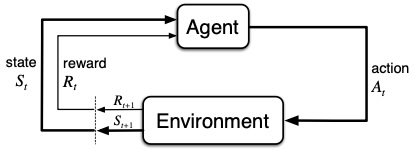
\includegraphics[width=\textwidth]{fig/agent_environment_interaction}}
\end{column}
\begin{column}{.2\textwidth}
\begin{itemize}
  \item Agente
  \item Acción
  \item Entorno
  \item Estado
  \item Recompensa
\end{itemize}
\end{column}
\end{columns}





\begin{columns}
\begin{column}{.50\textwidth}
\begin{itemize}
\item\textbf{ En cada paso $t$ el agente:}
	\begin{itemize}
	\item Recibe una \key{observación} $O_t$  y una recompensa $R_t$
	\item Ejecuta una \key{acción} $A_t$
	\end{itemize}
\end{itemize}
\end{column}
\begin{column}{.53\textwidth}
\begin{itemize}
\item \textbf{El entorno:}
	\begin{itemize}
	\item Recibe una \key{acción} $A_t$ y modifica su estado $S_t$ a $S_{t+1}$
	\item Emite una \key{observación} $O_{t+1}$ (y una recompensa $R_{t+1}$)
	\end{itemize}
\end{itemize}
\end{column}
\end{columns}

\vfill


    \begin{columns}
        \begin{column}{0.19\textwidth}
        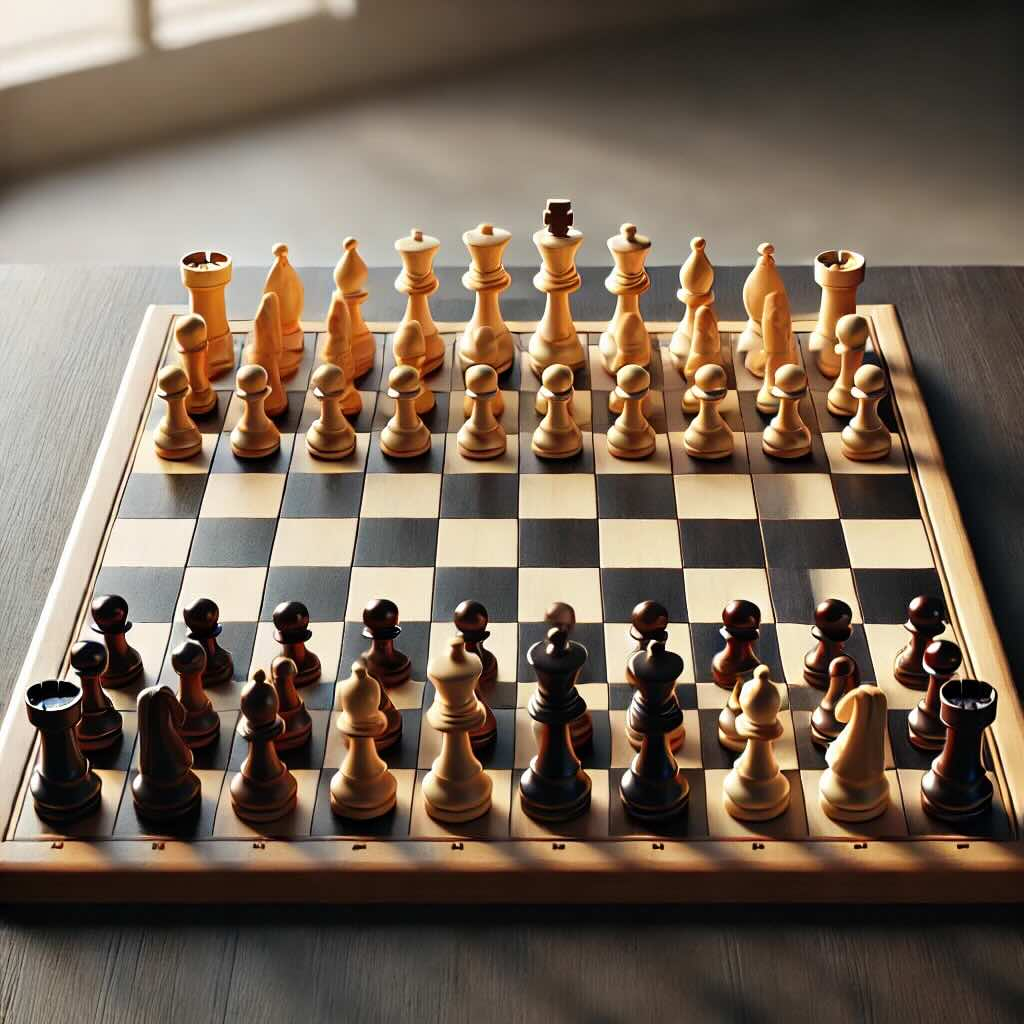
\includegraphics[width=\textwidth]{fig/ejedrez}
        \end{column}

        \begin{column}{0.19\textwidth}
        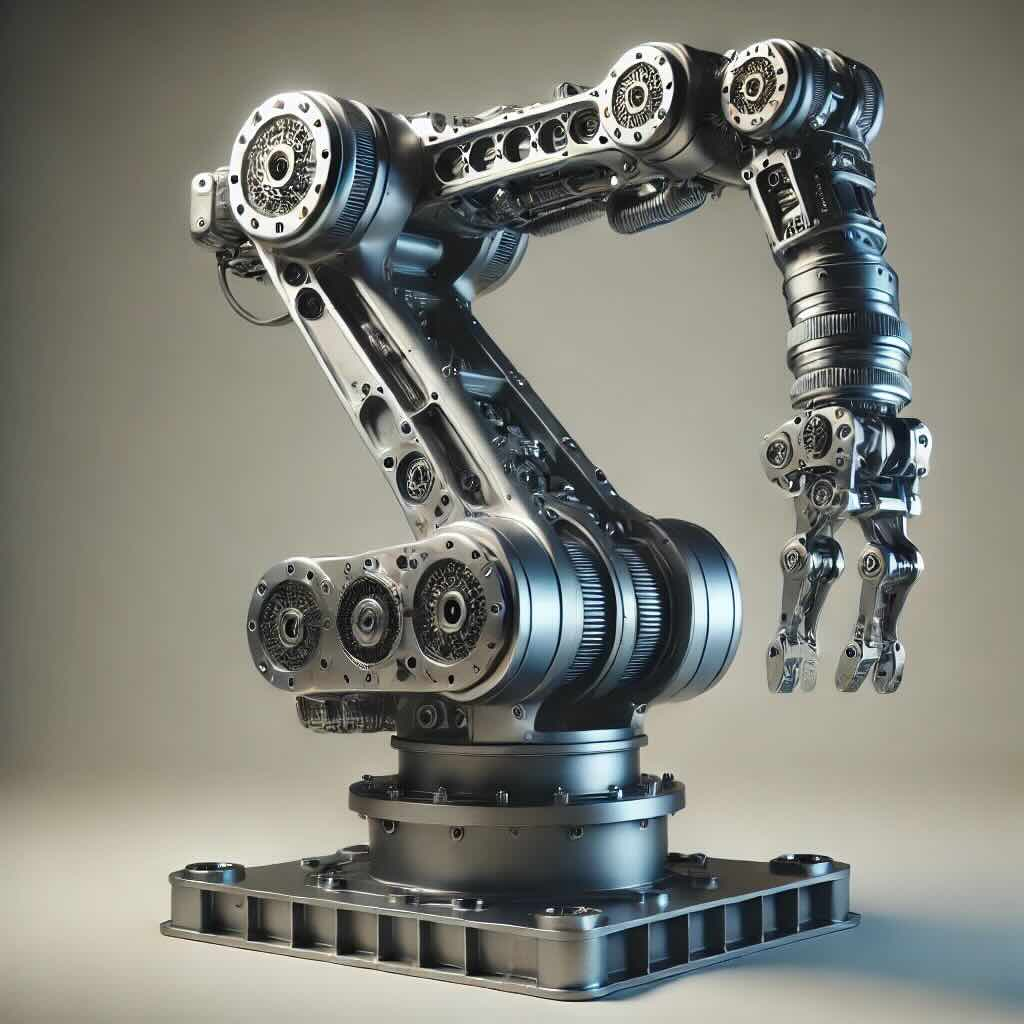
\includegraphics[width=\textwidth]{fig/robot}
        \end{column}

        \begin{column}{0.19\textwidth}
        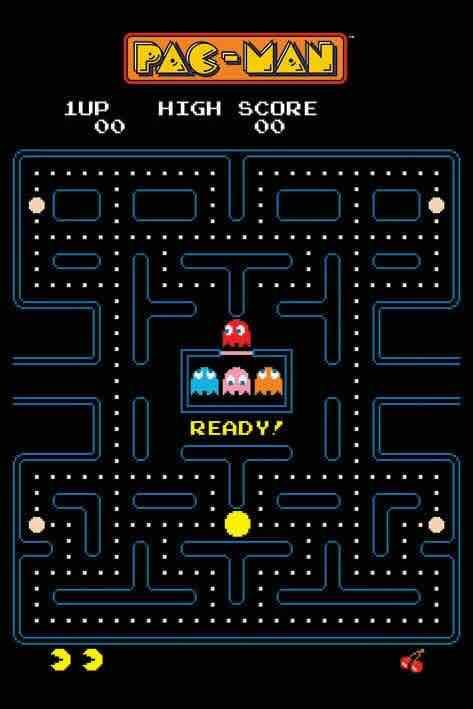
\includegraphics[width=\textwidth, height=.32\textheight]{fig/pac-man}
        \end{column}
    \end{columns}


\end{frame}


%%%%%%%%%%%%%%%%%%%%%%%%%%%%%%%%%%
%%%%%%%%%%%%%%%%%%%%%%%%%%%%%%%%%%

\subsection{Recompensas}

%%%%%%%%%%%%%%%%%%%%%%%%%%%%%%%%%%
%%%%%%%%%%%%%%%%%%%%%%%%%%%%%%%%%%
\begin{frame}{Recompensas}
\begin{itemize}
  \item \key{Recompensa:} Es una señal de retroalimentación escalar, $R_t\in\mathbb{R}$.
  
  \item Indica cómo de bien ha hecho la acción el agente.
  
  
  
  \item \key[red]{Hipótesis de la Recompensa}
  
  \begin{quote}\it
  Cualquier objetivo se puede formalizar como la maximización del valor esperado de la suma acumulada de las recompensas.
  \end{quote}
  
  \begin{itemize}
    \item El \key{retorno}, $G_t$, es la recompensa acumulada.
  
 	\hfil $G_t=R_{t+1}+R_{t+2}+R_{t+3}+\ldots$
	 
  \item El trabajo del agente es maximizar la recompensa acumulada.
  \end{itemize}
  

  \item Las recompensas se asignan por objetivos, no por subojetivos.
  
  
  \item \textbf{Ejemplos de Recompensas:}
    \begin{itemize}
      \item Ajedrez: Recompensa positiva por dar jaque mate, negativa si se comete un error que lleva al jaque mate del oponente, o cero si no ocurre ningún cambio significativo.
      \item Brazo robótico: Recompensa cero hasta que el objeto es correctamente manipulado, y positiva cuando el objetivo es alcanzado.
      \item Pac-Man: Recompensa positiva cuando el avatar come, negativas cuando no hace nada o lo comen.
    \end{itemize}
\end{itemize}


\end{frame}




%%%%%%%%%%%%%%%%%%%%%%%%%%%%%%%%%%
%%%%%%%%%%%%%%%%%%%%%%%%%%%%%%%%%%

\subsection{Acciones}


%%%%%%%%%%%%%%%%%%%%%%%%%%%%%%%%%%
%%%%%%%%%%%%%%%%%%%%%%%%%%%%%%%%%%
\begin{frame}{Acciones}
\begin{itemize}
  \item \key{Acción:} Las acciones, $A_t$, son las decisiones o movimientos que el agente puede tomar en un momento dado durante la tarea.
  	\begin{itemize}
	\item Vienen dadas por una \key{política} 
	\item La política del agente define su comportamiento y es un mapeo desde los estados a las acciones. 
	\item Dos casos: 
		\begin{itemize}
		\item Política determinista: $\pi(S)$
		\item Política estocástica, $\pi(A|S)=p(A|S)$
		\end{itemize}
	\end{itemize}

  \item Las acciones pueden tener \key{consecuencias} a largo plazo.

  \item Se adoptan con \key{el objetivo de maximizar el retorno}.
  	
  \item \textbf{Ejemplos de Acción:}
    \begin{itemize}
      \item Ajedrez: Movimiento de las piezas en el tablero.
      \item Brazo robótico: Modificación de la rotación de las juntas para manipular el objeto.
      \item Pac-Man: Pulsar los botones del mando para controlar el movimiento dtel avatar.
    \end{itemize}
\end{itemize}


\end{frame}



%%%%%%%%%%%%%%%%%%%%%%%%%%%%%%%%%%
%%%%%%%%%%%%%%%%%%%%%%%%%%%%%%%%%%

\subsection{Agente y  entorno}

%%%%%%%%%%%%%%%%%%%%%%%%%%%%%%%%%%
%%%%%%%%%%%%%%%%%%%%%%%%%%%%%%%%%%
\begin{frame}{El Agente y El Entorno}
\begin{itemize}
  \item \key{Agente:} Es la entidad que toma decisiones observando el estado del entorno y lleva a cabo las acciones en cada instante de tiempo.
  \begin{itemize}
  \item Ejemplos de Agentes:
    \begin{itemize}
      \item En ajedrez: el jugador humano que observa el estado de la partida y mueve las piezas.
      \item En el brazo robótico: el algoritmo que ajusta las juntas del brazo para manipular el objeto.
      \item En Pac-Man: el jugador o el sistema de IA que controla el avatar dentro del laberinto.
    \end{itemize}
  \end{itemize}
  
  \item \key{Entorno:} Incluye todos los elementos de la tarea que están fuera del control directo del agente.
  \begin{itemize}
  \item Ejemplos de Entorno:
    \begin{itemize}
      \item Ajedrez: El cronómetro y los movimientos del oponente.
      \item Brazo robótico: Factores físicos como la gravedad y la fricción de los objetos.
      \item Pac-Man: Los movimientos de los fantasmas y la disposición de las pastillas en el laberinto.
    \end{itemize}
  \end{itemize}
    
  \item Hay una interacción continua entre ellos.
    
 \centerline{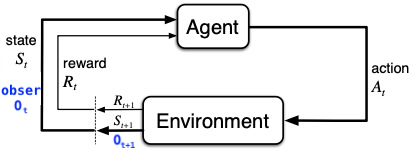
\includegraphics[width=0.5\textwidth]{fig/agent_environment_interaction2}}

\end{itemize}


\end{frame}



%%%%%%%%%%%%%%%%%%%%%%%%%%%%%%%%%%
%%%%%%%%%%%%%%%%%%%%%%%%%%%%%%%%%%

\subsection{Estados}

%%%%%%%%%%%%%%%%%%%%%%%%%%%%%%%%%%
%%%%%%%%%%%%%%%%%%%%%%%%%%%%%%%%%%
\begin{frame}{Estados}
\begin{itemize}
  \item La \key{historia} es la secuencia de observaciones, acciones y recompensas:
  \begin{equation*}
    H_t = O_1, R_1, A_1, \dots, A_{t-1}, O_t, R_t
  \end{equation*}
  \item Son todas las variables observables hasta el tiempo \( t \).
  \item Lo que sucede a continuación depende de la historia:
  \begin{itemize}
    \item El agente selecciona acciones.
    \item El entorno selecciona observaciones/recompensas.
  \end{itemize}
  \item El \key{estado} es la información utilizada para determinar lo que sucederá a continuación (por parte del agente/entorno).
  \item Formalmente, el estado es una función de la historia:
  \begin{equation*}
    S_t = f(H_t)
  \end{equation*} 
\end{itemize}



\end{frame}





%%%%%%%%%%%%%%%%%%%%%%%%%%%%%%%%%%
%%%%%%%%%%%%%%%%%%%%%%%%%%%%%%%%%%
\begin{frame}{Tipos de Estados}
\begin{itemize}

\item \key{Estado del Entorno}, $S_t^e$, es la representación privada del entorno.
\begin{itemize}
    \item Es cualquier dato que el entorno use para seleccionar la siguiente observación/recompensa.
    \item Normalmente no es visible para el agente. 
    \item Incluso si el conjunto $S_t^e$ fuese visible, puede contener información irrelevante.
\end{itemize}

\item \key{Estado del Agente}, $S_t^a$, es la representación interna del agente.
\begin{itemize}
\item Es cualquier información que el agente use para elegir la siguiente acción.
\item Es la información utilizada por los algoritmos de aprendizaje por refuerzo.
\item Puede ser cualquier función de la historia.
\end{itemize}

\TPMargin{0mm}%
\begin{textblock}{4.4}(11.4, 4.6)
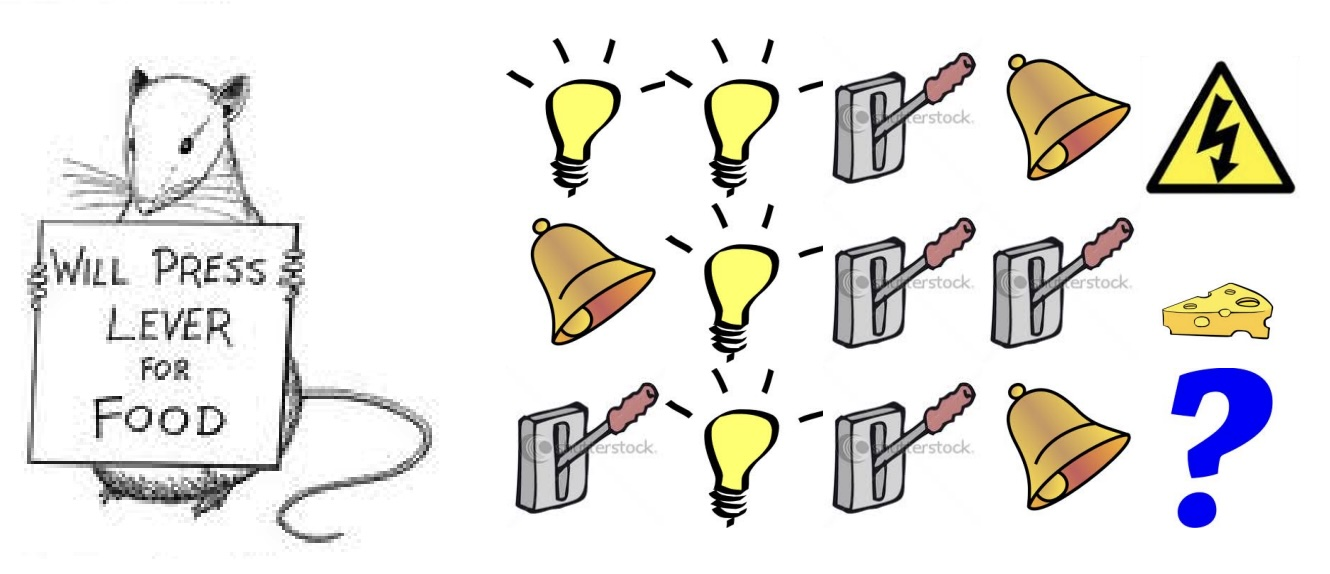
\includegraphics[width=\textwidth]{fig/ejemplo_rata}
\end{textblock}

\TPMargin{0mm}%
\begin{textblock}{4.4}(12.4, 9.0)

\includegraphics[width=.55\textwidth]{fig/dos_observaciones_lab}
\end{textblock}


\item \key{Estado Markoviano:} Es toda la información relevante para tomar una acción.  {\footnotesize $\mathbb{P}(S_{t+1}|S_t)=\mathbb{P}(S_{t+1}|S_1, \ldots S_t)$}

  
\item \key{¿Es observable?}
	\begin{itemize}
	\item \key{Completamente}: \(O_t = S^a_t = S^e_t\). 
	\item \key{Parcialmente}: El agente debe crear su propia representación $S^a_t$. 
		\begin{itemize}
		\item \textbf{Última observación}: \( S^a_t = O_t \) (puede no ser suficiente).
    	\item \textbf{Historia completa}: \( S^a_t = H_t \) (puede ser demasiado grande).
    	\item Algún estado actualizado \textbf{incrementalmente}: \( S^a_t = f(S_{t-1}, O_t) \).
		\item \textbf{Creencias sobre el estado del entorno}:\(S^a_t = (P[S^e_t = s_1], \dots, P[S^e_t = s_n]) \)
		\end{itemize}
	
	\end{itemize}
	
  
\item \textbf{Ejemplos de Estado:}
\begin{itemize}
  \item Ajedrez: Localización de las piezas en el tablero y el tiempo restante.
  \item Brazo robótico: Posición del objeto a manipular y la rotación de las juntas del brazo.
  \item Pac-Man: Posición del avatar, las pastillas amarillas y los fantasmas en el laberinto.
\end{itemize}
    
\end{itemize}


\end{frame}




%%%%%%%%%%%%%%%%%%%%%%%%%%%%%%%%%%
%%%%%%%%%%%%%%%%%%%%%%%%%%%%%%%%%%

\section{Otros Conceptos a Destacar}


%%%%%%%%%%%%%%%%%%%%%%%%%%%%%%%%%%
%%%%%%%%%%%%%%%%%%%%%%%%%%%%%%%%%%
\begin{frame}{Aprendizaje y Planificación. Predicción y Control.\\ Exploración y Explotación}
\begin{itemize}
\item Dos problemas fundamentales en la toma de decisiones secuencial:
    \begin{itemize}
    
        \item \key{Aprendizaje por Refuerzo}:
            \begin{itemize}
                \item El entorno es inicialmente desconocido.
                \item El agente interactúa con el entorno.
                \item El agente mejora su política.
            \end{itemize}
        \item \key{Planificación}:
            \begin{itemize}
                \item Se conoce un modelo del entorno.
                \item El agente realiza cálculos con el modelo (sin ninguna interacción externa).
                \item El agente mejora su política.
                \item También conocido como: deliberación, razonamiento, introspección, reflexión, búsqueda.
            \end{itemize}
    \end{itemize}
    

\TPMargin{0mm}%
\begin{textblock}{4.4}(11.4, 2.6)
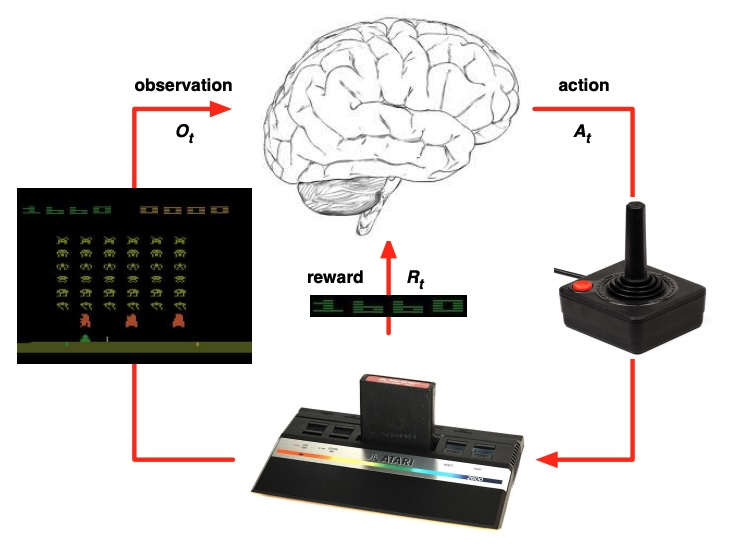
\includegraphics[width=\textwidth]{fig/aprender_atari}
\end{textblock}

\TPMargin{0mm}%
\begin{textblock}{4.4}(12, 9.0)
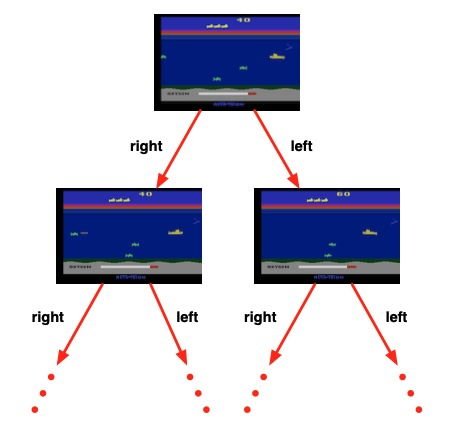
\includegraphics[width=.8\textwidth]{fig/planificar_atari}
\end{textblock}

   
\item Dos problemas fundamentales en el aprendizaje por refuerzo:
    \begin{itemize}
    
        \item \key{Explotación}: Utiliza la información conocida para maximizar la recompensa.
        \item \key{Exploración}: Encontrar más información sobre el entorno.
		\item Hay que buscar un equilibrio entre explorar y explotar.
    \end{itemize}
    
    
    
\item Dos conceptos muy relacionados: Predicción/Control.
	\begin{itemize}
        \item \key{Predicción}: evaluar el futuro (para una política dada).
        \item \key{Control}: optimizar el futuro (encontrar la mejor política).
        \item {Están fuertemente relacionados}. P.e:
        \(
        \pi_*(s) = \arg\max_{\pi} v_{\pi}(s)
        \)
    \end{itemize}
    
\end{itemize}


\end{frame}




%%%%%%%%%%%%%%%%%%%%%%%%%%%%%%%%%%
%%%%%%%%%%%%%%%%%%%%%%%%%%%%%%%%%%

\section{Una Taxonomía}

%%%%%%%%%%%%%%%%%%%%%%%%%%%%%%%%%%
%%%%%%%%%%%%%%%%%%%%%%%%%%%%%%%%%%


\begin{frame}{Tipos de Agentes}
\begin{itemize}
    \item \key{Política:} Determina cómo un agente decidirá una acción para un estado particular.
    \item \key{Función valor:} Especifica el valor esperado de acumulación de recompensas futuras desde un estado particular.
    \item \key{Modelos:} Representación del entorno que permite predecir el resultado de las acciones.
\end{itemize}

\begin{columns}
%%
\begin{column}{.4\textwidth}
\centerline{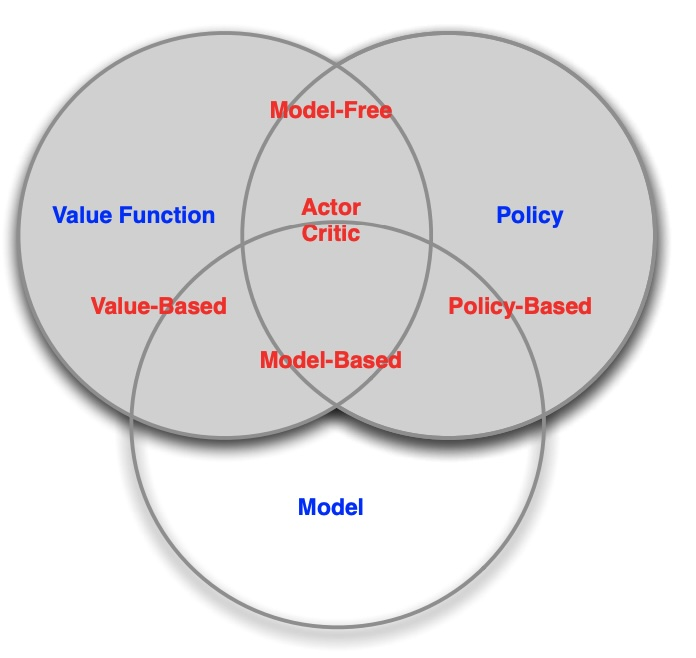
\includegraphics[width=\textwidth]{fig/taxonomia_agentes}}
\end{column}
%%
\begin{column}{.25\textwidth}
\begin{itemize}
\item {Basado en Valores}
    \begin{itemize}
        \item \textcolor{black!40}{Sin Política (Implícita)}
        \item Función de Valor
    \end{itemize}
            
\item {Basado en Políticas}
    \begin{itemize}
        \item Política
        \item \textcolor{black!40}{Sin Función de Valor}
    \end{itemize}

\item {Actor-Crítico}
    \begin{itemize}
        \item Política
        \item Función de Valor
    \end{itemize}
\end{itemize}
\end{column}
%%
\begin{column}{.25\textwidth}
\begin{itemize}
\item {Sin Modelo (Model-Free)}
    \begin{itemize}
        \item Política y/o Función de Valor
        \item \textcolor{black!40}{Sin Modelo}
	\end{itemize}
	
\item {Con Modelo (Model-Based)}
    \begin{itemize}
        \item Política y/o Función de Valor
        \item Con Modelo
    \end{itemize}
\end{itemize}
\end{column}
%%
\end{columns}



\end{frame}




%%%%%%%%%%%%%%%%%%%%%%%%%%%%%%%%%%
%%%%%%%%%%%%%%%%%%%%%%%%%%%%%%%%%%
\section{Conclusiones}

%%%%%%%%%%%%%%%%%%%%%%%%%%%%%%%%%%
%%%%%%%%%%%%%%%%%%%%%%%%%%%%%%%%%%
\begin{frame}{Conclusiones}
	
\begin{itemize}
	\item Comprensión de los elementos básicos (recompensas, acciones, estados, agente y entorno) es esencial.
	\item Los conceptos de exploración vs explotación se abordarán en el problema del bandido
	
	\item Los problemas de predicción vs control se irán estudiando en paralelo.
	
	\item La taxonomía proporcionan una base para estructurar los agentes  en RL.
	
	\item El aprendizaje por refuerzo es un campo con aplicaciones prácticas y teóricas amplias.
\end{itemize}
	
	
\end{frame}



%%%%%%%%%%%%%%%%%%%%%%%%%%%%%%%%%%
%%%%%%%%%%%%%%%%%%%%%%%%%%%%%%%%%%
% BIBLIOGRAFÍA
%%%%%%%%%%%%%%%%%%%%%%%%%%%%%%%%%%
%%%%%%%%%%%%%%%%%%%%%%%%%%%%%%%%%%


%%%%%%%%%%%%%%%%%%%%%%%%%%%%%%%%%%%%%%%%%%%%%%%%%%%%%%%%%%%%%%%%%%%%
%%%%%%%%%%%%%%%%%%%%%%%%%%%%%%%%%%%%%%%%%%%%%%%%%%%%%%%%%%%%%%%%%%%%

\section{Referencias}



% Redefinimos la apariencia
%\setbeamertemplate{headline}{}
%\setbeamertemplate{frametitle}{\vskip 0.5cm	\small{\textbf{\insertframetitle}}}
%\setbeamertemplate{footline}{}





% Mostramos la bibliografía
% \begin{frame}[allowframebreaks] %% Si ocupa más de una página
\begin{frame}[allowframebreaks]{Referencias -} %% Si hay sólo una página
	% \vskip -5cm %% Para ajustar la distancia al comienzo	
	%\bibliography{references}	
	\printbibliography[heading=none]
\end{frame}    


		
%%%%%%%%%%%%%%%%%%%%%%%%%%%%%%%%%%
%%%%%%%%%%%%%%%%%%%%%%%%%%%%%%%%%%

\end{document}

%%%%%%%%%%%%%%%%%%%%%%%%%%%%%%%%%%
%%%%%%%%%%%%%%%%%%%%%%%%%%%%%%%%%%
